\documentclass[a4]{scrartcl}

\usepackage{graphicx}
\usepackage{subcaption}

\title{Additional Results}

\begin{document}

\maketitle

\noindent
This document contains plots of the remaining posterior distributions that are not discussed in the main paper.

\begin{figure}[h]
  \centering
  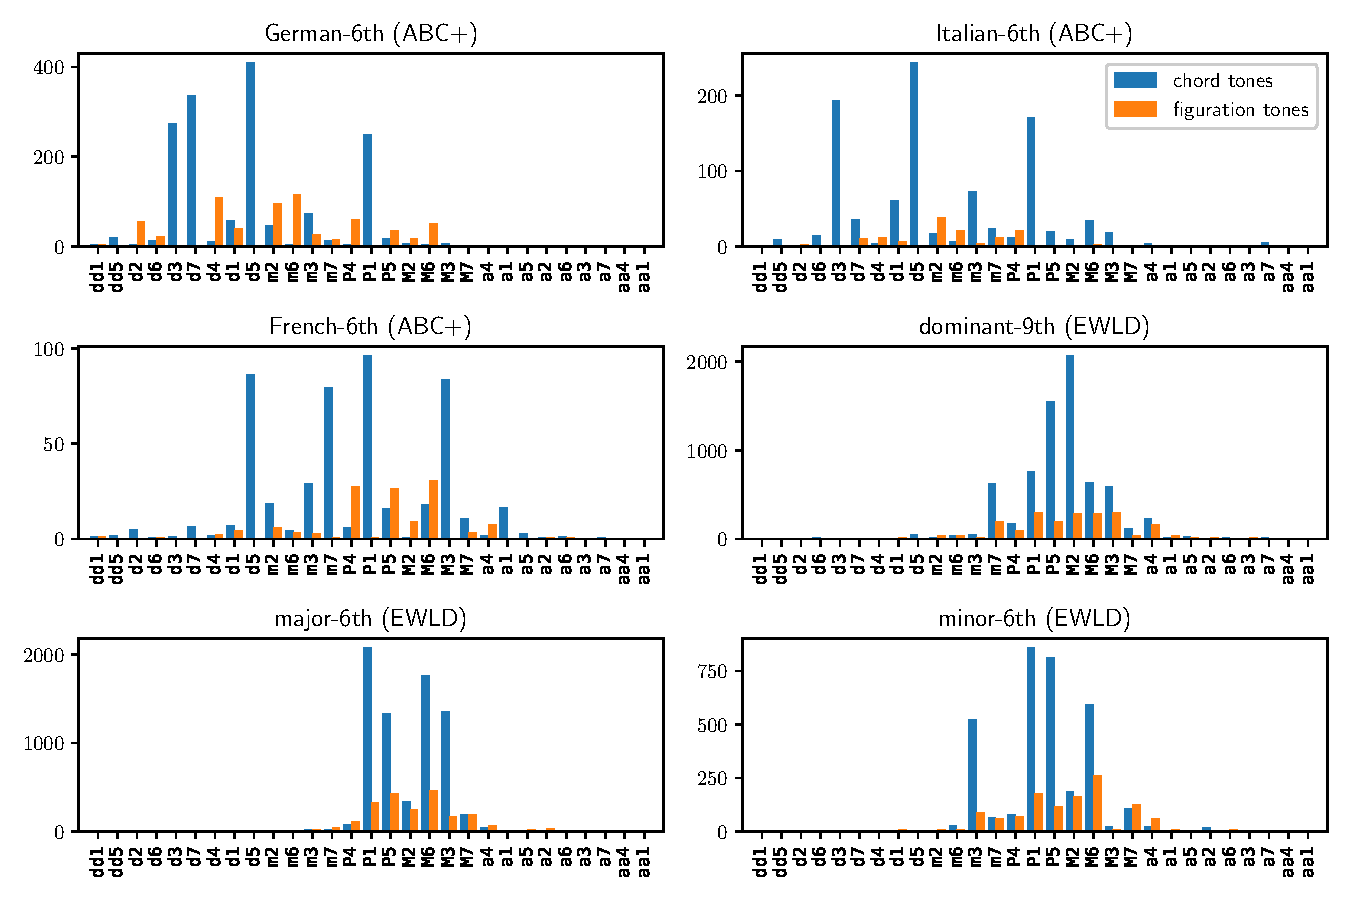
\includegraphics[width=\textwidth]{plots/chordtypes_rest1.pdf}
  \caption[The posterior distributions of the chordtones $\phi^{(ct)}$ and ornaments $\phi^{(or)}$
    of the chord types that are specific to either the ABC+ or the EWLD corpus.]{
    The posterior distributions of the chordtones $\phi^{(ct)}$ (blue, left-leaning bars)
    and ornaments $\phi^{(or)}$ (orange, right-leaning bars)
    of the chord types that are specific to either the ABC+ or the EWLD corpus.
    The chords that are common to both datasets are shown in the main paper.
    Pitches are ordered according to the line of fifths
    and expressed as intervals relative to the root (P1, unison).
    (Continues on next page.)
  }
  \label{fig:harmonies-ornaments.profiles-rest}
\end{figure}%
\begin{figure}\ContinuedFloat
  \centering
  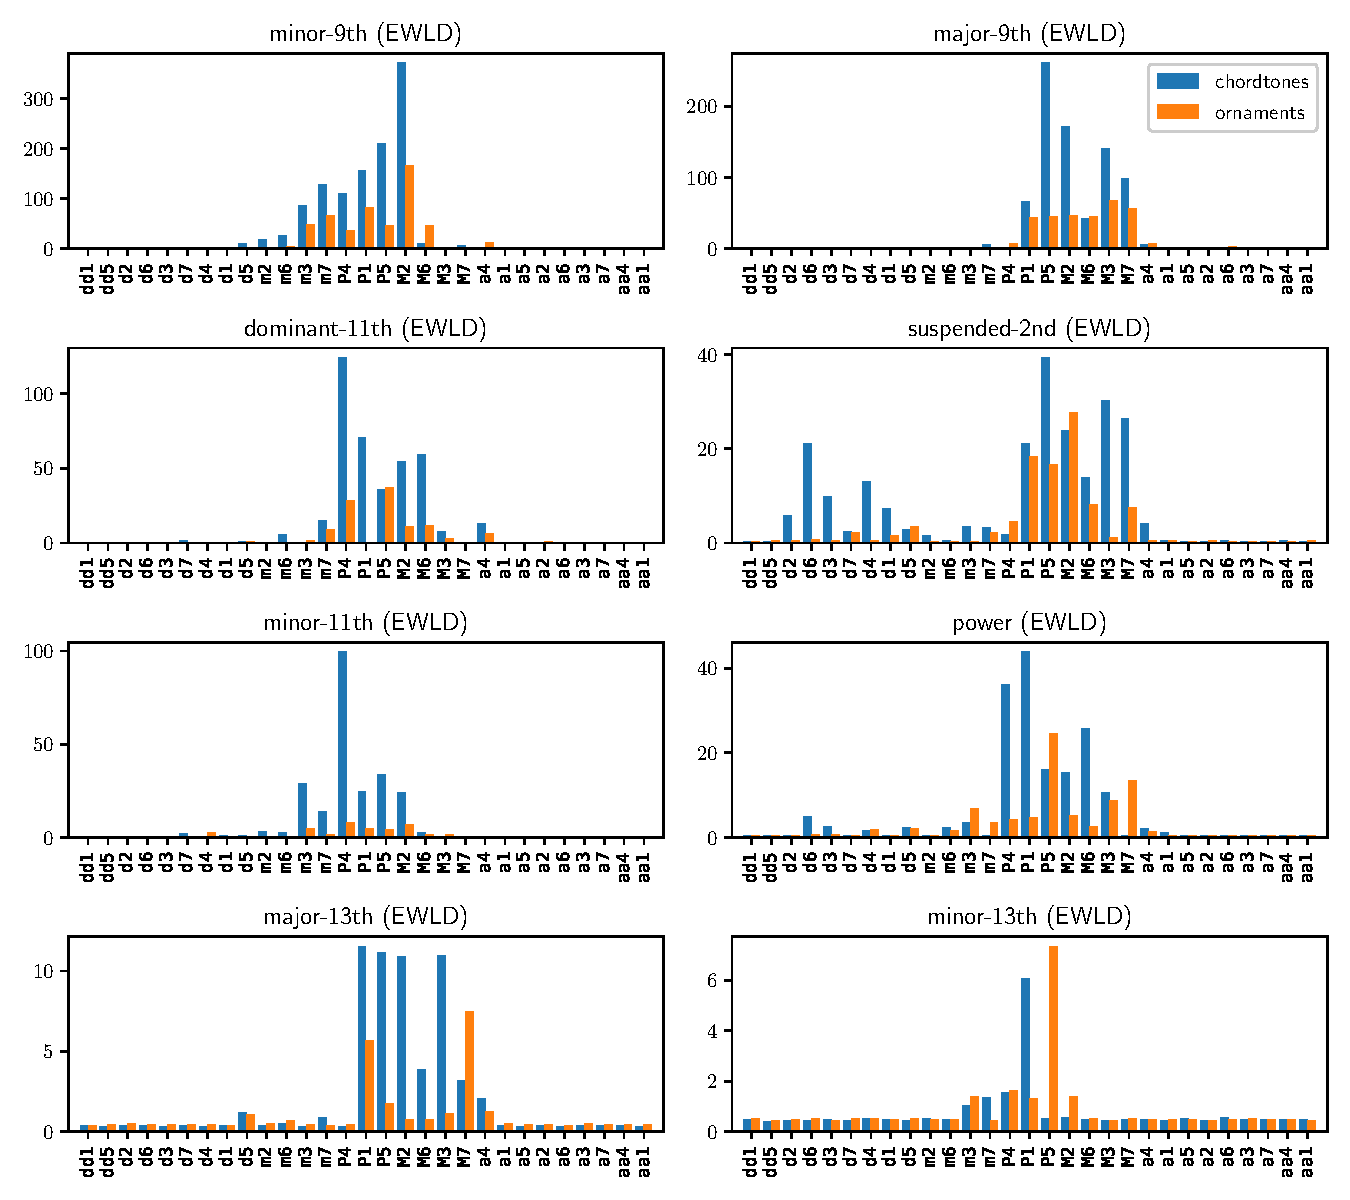
\includegraphics[width=\textwidth]{plots/chordtypes_rest2.pdf}
  \caption[]{(cont.)}
\end{figure}

\begin{figure}[h]
  \centering
  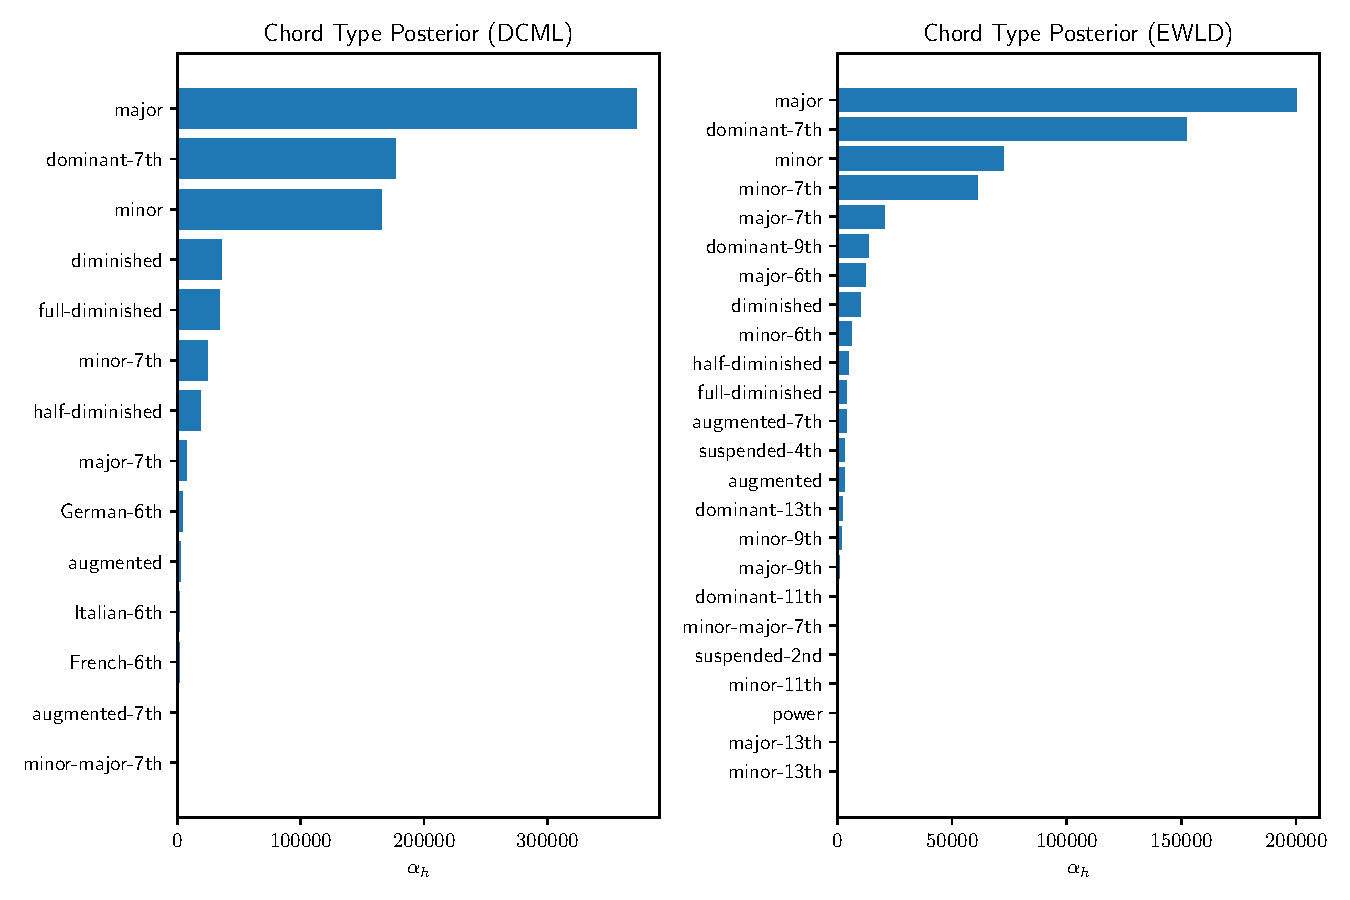
\includegraphics[width=\textwidth]{plots/type_dist.pdf}
  \caption[Posterior distributions of the chord type probabilities $\chi$.]{
    Posterior distributions of the chord type probabilities $\chi$.
    The bars indicate the parameters of the posterior Dirichlet distribution,
    where one parameter corresponds to each chord type and indicates the prevalence of that chord type.
    The values essentially correspond to the number of occurrences of each chord types.
  }
  \label{fig:harmonies-ornaments.post-types}
\end{figure}

\begin{figure}[h]
  \centering
  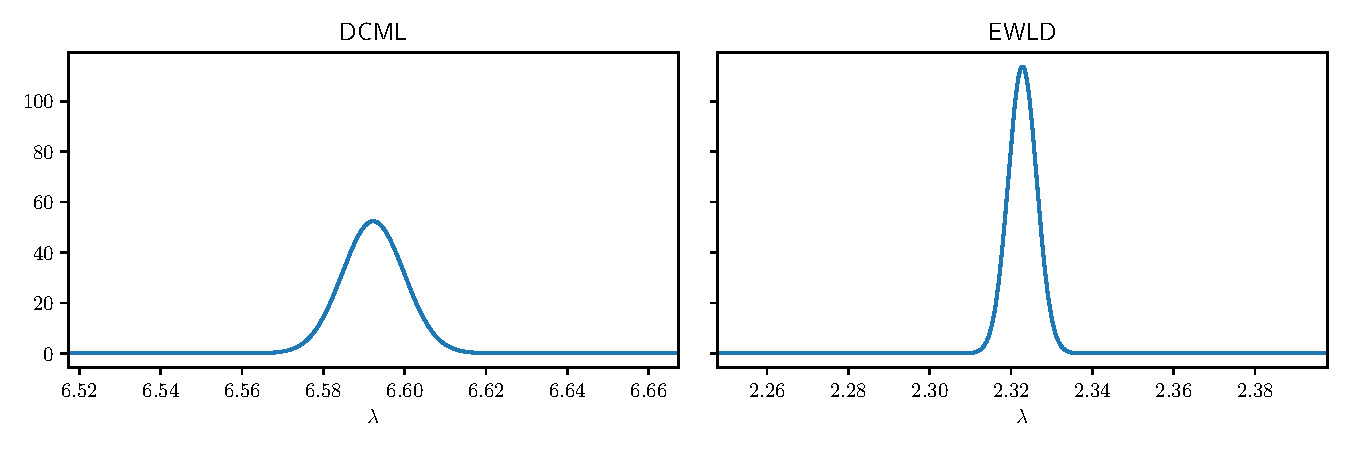
\includegraphics[width=\textwidth]{plots/note_rates.pdf}
  \caption[Posterior distributions of the note rate $\lambda$.]{
    Posterior distributions of the note rate $\lambda$
    for the ABC+ corpus (left) and the EWLD corpus (right).
    Both plots share the y-axis and have the same scaling on the x-axis,
    so the variance of the distrubtions can be compared directly.
    The mean, however, is much smaller for the EWLD data,
    probably due to the fact that it consists of melodies instead of full scores.
  }
  \label{fig:harmonies-ornaments.post-rates}
\end{figure}


% \section{Remaining Chord-Type Profiles}

% The posterior distributions of the chordtones $\phi^{(ct)}$ (blue, left-leaning bars)
% and ornaments $\phi^{(or)}$ (orange, right-leaning bars)
% of the chord types that are specific to either the ABC+ or the EWLD corpus.
% The chords that are common to both datasets are shown in the main paper.
% Pitches are ordered according to the line of fifths
% and expressed as intervals relative to the root (P1, unison).

% 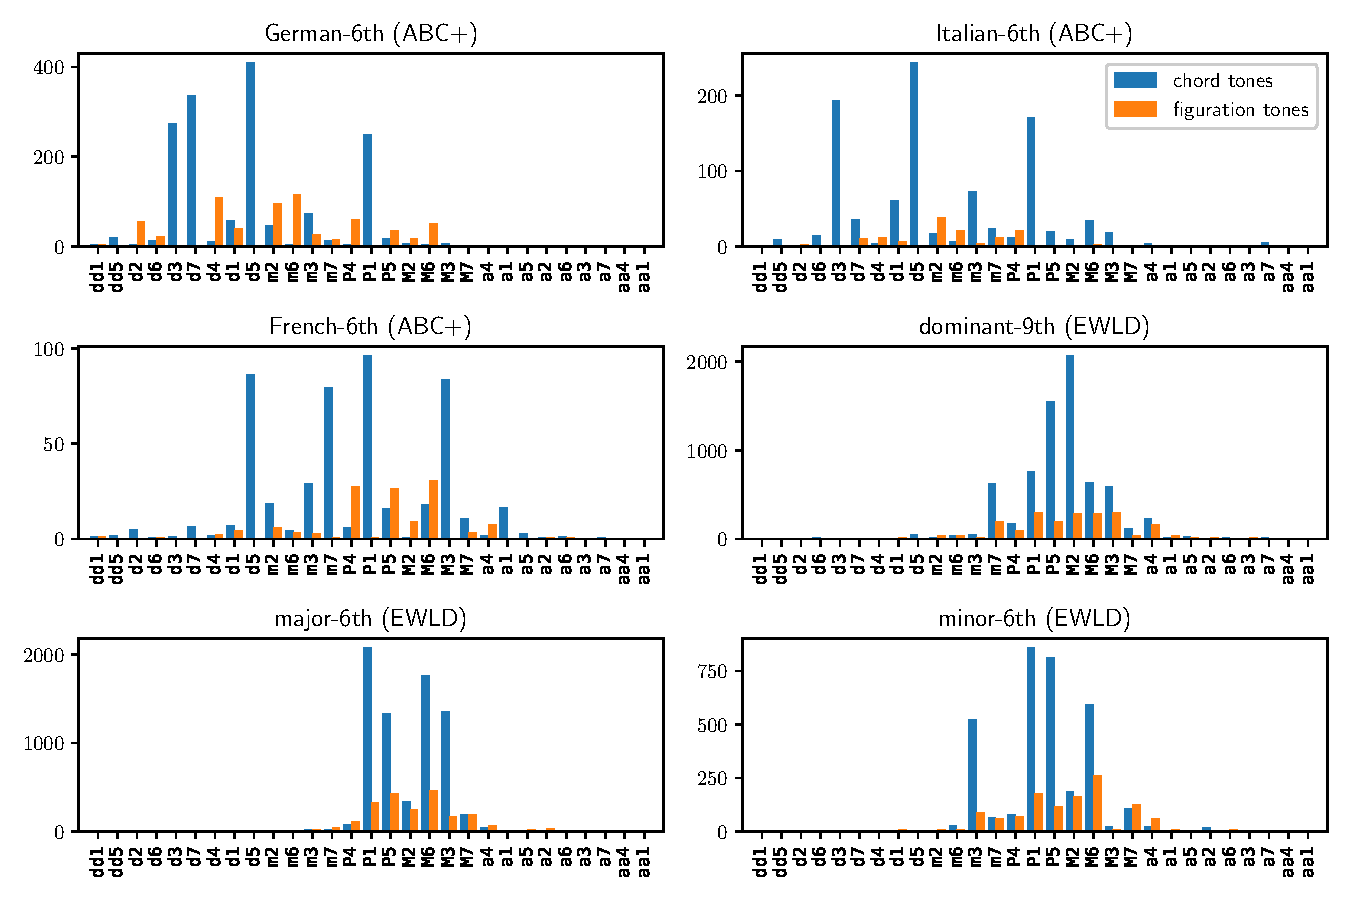
\includegraphics[width=\textwidth]{plots/chordtypes_rest1.pdf}

% 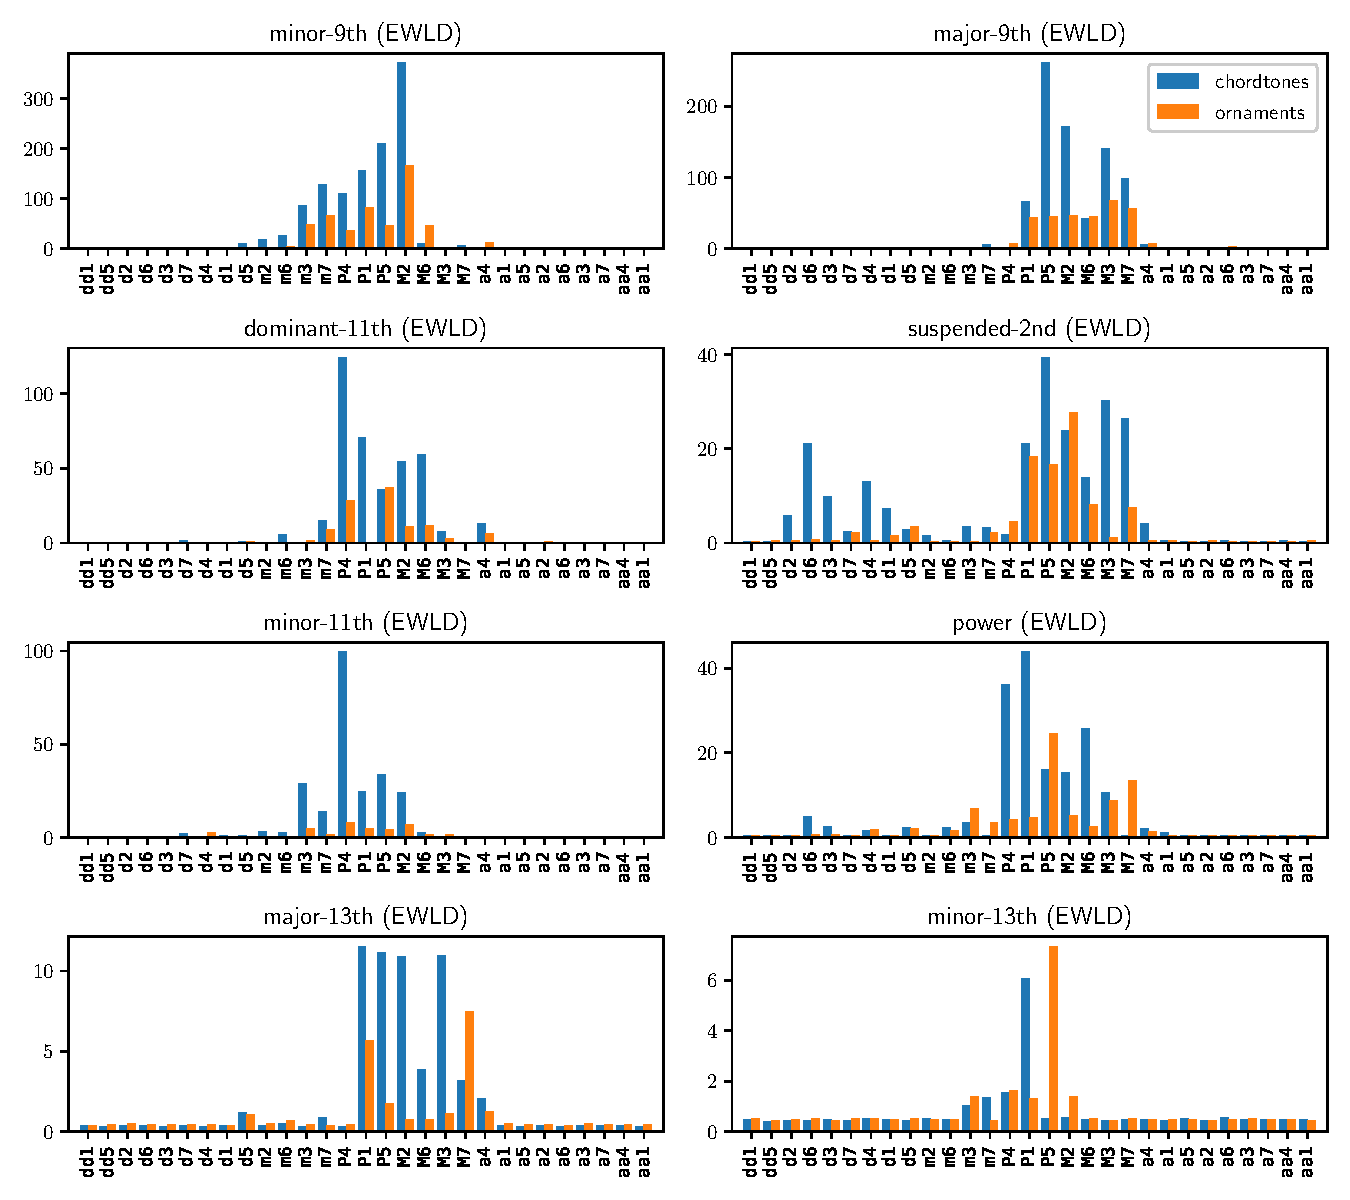
\includegraphics[width=\textwidth]{plots/chordtypes_rest2.pdf}

% \clearpage
% \section{Chord Type Probabilities}

% Posterior distributions of the chord type probabilities $\chi$.
% The bars indicate the parameters of the posterior Dirichlet distribution,
% where one parameter corresponds to each chord type and indicates the prevalence of that chord type.
% The values essentially correspond to the number of occurrences of each chord types.

% 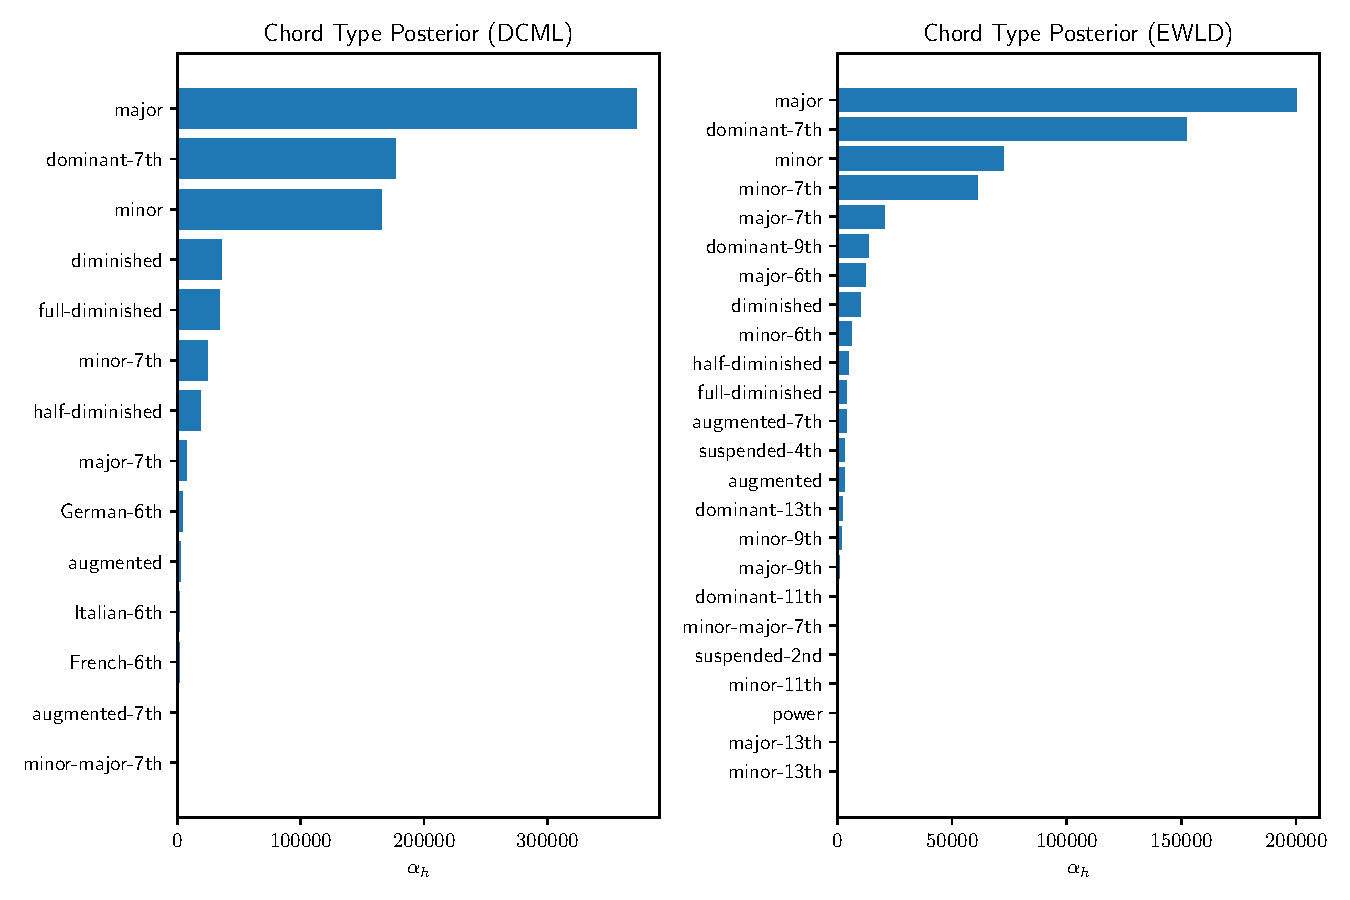
\includegraphics[width=\textwidth]{plots/type_dist.pdf}

% \clearpage
% \section{Note Rates}

% Posterior distributions of the note rate $\lambda$
% for the ABC+ corpus (left) and the EWLD corpus (right).
% Both plots share the y-axis and have the same scaling on the x-axis,
% so the variance of the distrubtions can be compared directly.
% The mean, however, is much smaller for the EWLD data,
% probably due to the fact that it consists of melodies instead of full scores.

% 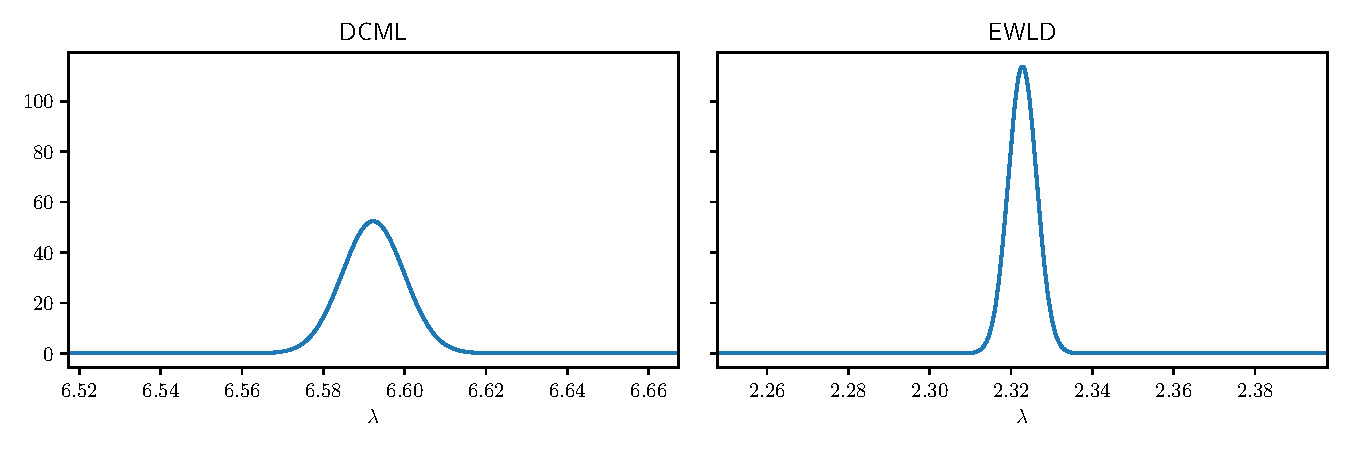
\includegraphics[width=\textwidth]{plots/note_rates.pdf}

\end{document}